\documentclass[letterpaper, 10 pt, conference]{ieeeconf}

\IEEEoverridecommandlockouts 
\overrideIEEEmargins
%\documentclass[letterpaper, 12pt, draftcls, onecolumn]{IEEEtran}

% Mathematical Tools
\usepackage{amsmath}
\usepackage{amssymb, amsfonts}
\usepackage{booktabs} 
\usepackage{mathtools}
\usepackage{commath}
\usepackage{microtype}

%\usepackage{amsthm}
\usepackage{mathdots}
\usepackage{mathtools}
\usepackage{bm}

\usepackage{eucal}


% TIKZ package 
\usepackage{tikz}
\usepackage{pgfplots}
\pgfplotsset{every axis/.append style={line width=1pt}}
\pgfplotsset{compat=newest}
\usetikzlibrary{shapes, fit, decorations.markings, matrix, plotmarks, positioning, fit, spy, patterns, shadows, calc, backgrounds, arrows.meta}



% figures
\usepackage[font=footnotesize,caption=false]{subfig}
\usepackage{graphicx}
\usepackage[abs]{overpic}

% input
\usepackage{inputenc}
\usepackage[nolist]{acronym}
\usepackage{siunitx}
\usepackage{booktabs}


% enumerate and equations
\usepackage{enumerate}
%\AtBeginEnvironment{align}{\setcounter{subeqn}{0}}% Reset subequation number at start of align
\newcounter{subeqn} \renewcommand{\thesubeqn}{\theequation\alph{subeqn}}%
\newcommand{\subeqn}{%
  \refstepcounter{subeqn}% Step subequation number
  \tag{\thesubeqn}% Label equation
}


% Theorems
\newtheorem{theorem}{Theorem}
\newtheorem{corollary}{Corollary}
\newtheorem{lemma}[theorem]{Lemma}
\newtheorem{proposition}{Proposition}
\newtheorem{assumption}{Assumption}
\newtheorem{definition}{Definition}
\newtheorem{alg}{Algorithm}[section]
\newtheorem{example}{Example}
\newtheorem{remark}{Remark}
\newtheorem{problem}{Problem}


% Create shorthand definitions
\newcommand{\ts}[1]{{\textnormal{#1}}}
\newcommand{\ie}{\emph{i.e.}\ }
\newcommand{\eg}{\emph{e.g.}}
\newcommand{\cf}{\emph{c.f.}\ }
\newcommand{\Nset}{\mathbb{N}}
\newcommand{\Rset}{\mathbb{R}}
\newcommand{\Cset}{\mathbb{C}}
\newcommand{\mc}{\mathcal}
\newcommand{\mb}{\mathbf}
\newcommand{\mbb}{\mathbb}
\newcommand{\mf}{\mathfrak}
\newcommand{\ms}{\mathscr}

\def\vv{\vspace{1mm}}
\def\vs{\vspace{\baselineskip}}
\newcommand{\edit}[1]{\textcolor{blue}{#1}}

\newcommand{\diff}[2]{{\frac{d #1}{d #2}}}
\newcommand{\pdiff}[2]{{\frac{\partial #1}{\partial #2}}}

% Activate selected proofs
\newif\ifproves
\provestrue

\allowdisplaybreaks

\begin{acronym}
	\acro{MPC}{Model Predictive Control}
	\acro{DMPC}{Distributed Model Predictive Control}
	\acro{LSS}{Large-Scale System}
	\acro{mRPI}{minimal Robust Positively Invariant}
	\acro{QP}{Quadratic Programming}
	\acro{RCI}{Robust Control Invariant}
	\acro{RPI}{Robust Positive Invariant}
	\acro{PnP}{Plug and Play}
	\acro{OCP}{Optimal Control Problem}
	\acro{MPC}{Model Predictive Control}
	\acro{PV}{Photo-voltaic}
	\acro{DG}{Distributed Generation}
	\acro{DS}{Distributed Storage}
	\acro{BIC}{Bounded Integral Controller}
	\acro{VCS}{Voltage controlled source}
	\acro{MG}{Microgrid}
	\acro{OPF}{Optimal Power Flow}
	\acro{SoC}{State of Charge}
	\acro{OCP}{Optimal Control Problem}
	\acro{CPL}{Constant Power Load}		
\end{acronym}
%
\interdisplaylinepenalty=2500
%

% bibliography
\usepackage{cite}
\bibliographystyle{IEEEtran}


% Required in the preamble
% % % % % % % % % % % % % % % % % % % % % % % % % % % %
% % % % % % % % % % % % % % % % % % % % % % % % % % % %
% % % % % % % % % % % % % % % % % % % % % % % % % % % %
% defining the new dimensions and parameters
\newlength{\hatchspread}
\newlength{\hatchthickness}
\newlength{\hatchshift}
\newcommand{\hatchcolor}{}
% declaring the keys in tikz
\tikzset{hatchspread/.code={\setlength{\hatchspread}{#1}},
         hatchthickness/.code={\setlength{\hatchthickness}{#1}},
         hatchshift/.code={\setlength{\hatchshift}{#1}},% must be >= 0
         hatchcolor/.code={\renewcommand{\hatchcolor}{#1}}}
% setting the default values
\tikzset{hatchspread=3pt,
         hatchthickness=0.4pt,
         hatchshift=0pt,% must be >= 0
         hatchcolor=black}
% declaring the pattern
\pgfdeclarepatternformonly[\hatchspread,\hatchthickness,\hatchshift,\hatchcolor]% variables
   {nwl}% name
   {\pgfqpoint{\dimexpr-2\hatchthickness}{\dimexpr-2\hatchthickness}}% lower left corner
   {\pgfqpoint{\dimexpr\hatchspread+2\hatchthickness}{\dimexpr\hatchspread+2\hatchthickness}}% upper right corner
   {\pgfqpoint{\dimexpr\hatchspread}{\dimexpr\hatchspread}}% tile size
   {% shape description
    \pgfsetlinewidth{\hatchthickness}
    \pgfpathmoveto{\pgfqpoint{0pt}{\dimexpr\hatchspread+\hatchshift}}
    \pgfpathlineto{\pgfqpoint{\dimexpr\hatchspread+0.15pt+\hatchshift}{-0.15pt}}
    \ifdim \hatchshift > 0pt
      \pgfpathmoveto{\pgfqpoint{0pt}{\hatchshift}}
      \pgfpathlineto{\pgfqpoint{\dimexpr0.15pt+\hatchshift}{-0.15pt}}
    \fi
    \pgfsetstrokecolor{\hatchcolor}
%    \pgfsetdash{{1pt}{1pt}}{0pt}% dashing cannot work correctly in all situation this way
    \pgfusepath{stroke}
   }
\pgfdeclarepatternformonly[\hatchspread,\hatchthickness,\hatchshift,\hatchcolor]% variables
   {nwld}% name
   {\pgfqpoint{\dimexpr-2\hatchthickness}{\dimexpr-2\hatchthickness}}% lower left corner
   {\pgfqpoint{\dimexpr\hatchspread+2\hatchthickness}{\dimexpr\hatchspread+2\hatchthickness}}% upper right corner
   {\pgfqpoint{\dimexpr\hatchspread}{\dimexpr\hatchspread}}% tile size
   {% shape description
    \pgfsetlinewidth{\hatchthickness}
    \pgfpathmoveto{\pgfqpoint{0pt}{\dimexpr\hatchspread+\hatchshift}}
    \pgfpathlineto{\pgfqpoint{\dimexpr\hatchspread+0.15pt+\hatchshift}{-0.15pt}}
    \ifdim \hatchshift > 0pt
      \pgfpathmoveto{\pgfqpoint{0pt}{\hatchshift}}
      \pgfpathlineto{\pgfqpoint{\dimexpr0.15pt+\hatchshift}{-0.15pt}}
    \fi
    \pgfsetstrokecolor{\hatchcolor}
    \pgfsetdash{{1pt}{1pt}}{0pt}% dashing cannot work correctly in all situation this way
    \pgfusepath{stroke}
   }
\pgfdeclarepatternformonly[\hatchspread,\hatchthickness,\hatchshift,\hatchcolor]% variables
   {nel}% name
   {\pgfqpoint{\dimexpr-2\hatchthickness}{\dimexpr-2\hatchthickness}}% lower left corner
   {\pgfqpoint{\dimexpr\hatchspread+2\hatchthickness}{\dimexpr\hatchspread+2\hatchthickness}}% upper right corner
   {\pgfqpoint{\dimexpr\hatchspread}{\dimexpr\hatchspread}}% tile size
   {% shape description
    \pgfsetlinewidth{\hatchthickness}
    \pgfpathmoveto{\pgfqpoint{\dimexpr\hatchshift-0.15pt}{-0.15pt}}
    \pgfpathlineto{\pgfqpoint{\dimexpr\hatchspread+0.15pt}{\dimexpr\hatchspread-\hatchshift+0.15pt}}
    \ifdim \hatchshift > 0pt
      \pgfpathmoveto{\pgfqpoint{-0.15pt}{\dimexpr\hatchspread-\hatchshift-0.15pt}}
      \pgfpathlineto{\pgfqpoint{\dimexpr\hatchshift+0.15pt}{\dimexpr\hatchspread+0.15pt}}
    \fi
    \pgfsetstrokecolor{\hatchcolor}
%    \pgfsetdash{{1pt}{1pt}}{0pt}% dashing cannot work correctly in all situation this way
    \pgfusepath{stroke}
   }
\pgfdeclarepatternformonly[\hatchspread,\hatchthickness,\hatchshift,\hatchcolor]% variables
   {neld}% name
   {\pgfqpoint{\dimexpr-2\hatchthickness}{\dimexpr-2\hatchthickness}}% lower left corner
   {\pgfqpoint{\dimexpr\hatchspread+2\hatchthickness}{\dimexpr\hatchspread+2\hatchthickness}}% upper right corner
   {\pgfqpoint{\dimexpr\hatchspread}{\dimexpr\hatchspread}}% tile size
   {% shape description
    \pgfsetlinewidth{\hatchthickness}
    \pgfpathmoveto{\pgfqpoint{\dimexpr\hatchshift-0.15pt}{-0.15pt}}
    \pgfpathlineto{\pgfqpoint{\dimexpr\hatchspread+0.15pt}{\dimexpr\hatchspread-\hatchshift+0.15pt}}
    \ifdim \hatchshift > 0pt
      \pgfpathmoveto{\pgfqpoint{-0.15pt}{\dimexpr\hatchspread-\hatchshift-0.15pt}}
      \pgfpathlineto{\pgfqpoint{\dimexpr\hatchshift+0.15pt}{\dimexpr\hatchspread+0.15pt}}
    \fi
    \pgfsetstrokecolor{\hatchcolor}
    \pgfsetdash{{1pt}{1pt}}{0pt}% dashing cannot work correctly in all situation this way
    \pgfusepath{stroke}
   }
% % % % % % % % % % % % % % % % % % % % % % % % % % % %
% % % % % % % % % % % % % % % % % % % % % % % % % % % %
% % % % % % % % % % % % % % % % % % % % % % % % % % % %
%===============================================================================


\title{Title here}
%

%\markboth{IEEE Transactions on Automatic Control}{}

%\IEEEpubid{0000--0000/00\$00.00~\copyright~2015 IEEE}

\author{Pablo R. Baldivieso-Monasterios$^{1}$
\thanks{P.R. Baldivieso-Monasterios is with the Department of Automatic Control \& Systems Engineering, University of Sheffield, Sheffield, UK {\tt\small \{p.baldivieso\}@sheffield.ac.uk}.}
}
\begin{document}
	%
\maketitle
		%
\begin{abstract}            
stuff happens here
\end{abstract}
%

\section{Introduction}
\label{sec:introduction}

\cite{Limon2009}
%\newcommand{\myreferences}{/Users/Pablo/Dropbox/Reports/library}
%\newcommand{\myreferences}{/Users/prbalm/Dropbox/Reports/library.bib}
%\newcommand{\myreferences}{extracted}
%\newcommand{\myreferences}{library}

\begin{figure}[b!]
  \centering
  % This file was created by matlab2tikz.
% Minimal pgfplots version: 1.3
%
\definecolor{mycolor1}{rgb}{0.00000,0.44700,0.74100}%
\definecolor{mycolor2}{rgb}{0.85000,0.32500,0.09800}%
\definecolor{mycolor3}{rgb}{0.92900,0.69400,0.12500}%
\definecolor{mycolor4}{rgb}{0.49400,0.18400,0.55600}%
\definecolor{mycolor5}{rgb}{0.46600,0.67400,0.18800}%
\definecolor{mycolor6}{rgb}{0.30100,0.74500,0.93300}%
\definecolor{mycolor7}{rgb}{0.63500,0.07800,0.18400}%
%
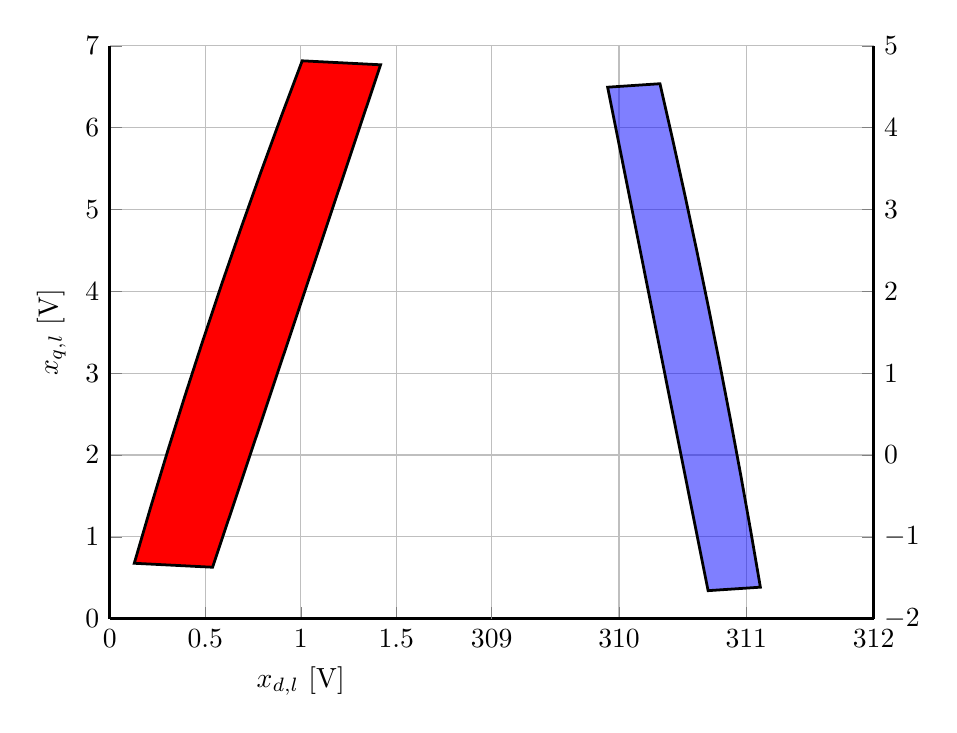
\begin{tikzpicture}


\begin{axis}[%
width=0.4\linewidth,
height=0.6\linewidth,
at={(0\linewidth,0\linewidth)},
scale only axis,
xmin=0,
xmax=2,
ymin=0,
ymax=7,
axis x line*=bottom,
axis y line*=left,
xmajorgrids,
ymajorgrids,
xlabel={$x_{d,l}$ [\si{\volt}]},
xtick={  0, 0.5, 1, 1.5},
ylabel={$x_{q,l}$ [\si{\volt}]},
legend style={legend cell align=left,align=left,draw=white!15!black}
]

\addplot[area legend,solid,line width=1.0pt,fill=red,draw=black]
table[row sep=crcr] {%
x	y	z\\
0.538001295287672	0.628344671185063	\\
0.492384649139163	0.633740803488589	\\
0.44678160003676	0.639136835572078	\\
0.401192135986202	0.644532767523937	\\
0.355616245010898	0.649928599432442	\\
0.310053915151885	0.655324331385739	\\
0.264505134467795	0.660719963471844	\\
0.218969891034816	0.666115495778645	\\
0.173448172946662	0.671510928393899	\\
0.127939968314528	0.676906261405236	\\
0.213424740000106	1.35918535295086	\\
0.301953292663312	2.04144200963536	\\
0.393530537543134	2.72367619525937	\\
0.488161576362579	3.40588787221951	\\
0.585851702864203	4.08807700149709	\\
0.686606404409384	4.77024354264627	\\
0.79043136364249	5.45238745378189	\\
0.897332460221152	6.13450869156663	\\
1.00731577261388	6.81660721119777	\\
1.41778191248323	6.76804263721459	\\
}--cycle;\label{fig:eq_1}

\end{axis}

\begin{axis}[%
width=0.4\linewidth,
height=0.6\linewidth,
at={(0.4\linewidth,0.0\linewidth)},
scale only axis,
%every outer x axis line/.append style={white!10!black},
%every x tick label/.append style={font=\color{white!10!black}},
%legend style={draw=none,at={(0.6,1.30)},anchor=north,legend columns=-1},
xmin=309,
xmax=312,
ymin=-2,
ymax=5,
%xmin=0,
%xmax=100,
%xtick={  0, 15, 25, 45, 65 ,90, 100},
%tick align=outside,
%xlabel={$u_{d,l}$ [\si{\ampere}]},
%ylabel={$u_{q,l}$ [\si{\ampere}]},
xmajorgrids,
%every outer y axis line/.append style={white!10!black},
%every y tick label/.append style={font=\color{white!10!black}},
%ymin=-50,
%ymax=80,
%ytick={-50,0,70},
%yticklabels={$-S_b$,$0$,$Sb$,$S_w$},
ymajorgrids,
axis x line*=bottom,
axis y line*=right
]

\addplot[area legend,solid,line width=1.0pt,fill=blue,draw=black, fill opacity = 0.5]
table[row sep=crcr] {%
x	y\\
310.95642599536	-0.248305512318877\\
311.034888028568	-0.931793010062459\\
311.110306280799	-1.61525807294492	\\
311.064723489924	-1.61998199962041\\
311.019127185594	-1.62470582669197	\\
310.973517355918	-1.62942955407199	\\
310.927893988992	-1.63415318167271	\\
310.882257072891	-1.63887670940623	\\
310.836606595673	-1.64360013718455	\\
310.79094254538	-1.64832346491951	\\
310.745264910035	-1.65304669252285	\\
310.699573677644	-1.65776981990614	\\
309.910391735543	4.49422960391711	\\
310.321529151594	4.53673836711531	\\
310.421445944532	3.85309273231837	\\
310.518280521655	3.16946981567502	\\
310.612038961434	2.48586957238255	\\
310.702727143524	1.80229195910366	\\
310.790350750571	1.11873693395314	\\
310.874915269935	0.435204456485197	\\
}--cycle;\label{fig:eq_2}
\end{axis}
\end{tikzpicture}%
  \caption{trial}
  \label{fig:trial}
\end{figure}

\bibliography{extracted}

\end{document}
%%% Local Variables:
%%% mode: latex
%%% TeX-master: t
%%% End:
